%%==================================================================%%
%% Author : Sa�udo Olmedo, Ignacio                                  %%
%%          S�nchez Barreiro, Pablo                                 %%
%% Version: 2.2, 18/06/2014                                         %%                                                                                    %%                                                                  %%
%% Memoria del Proyecto Fin de Carrera                              %%
%% Archivo ra�z                                                     %%
%%==================================================================%%

\chapterheader{Introducci�n}{Introducci�n}
\label{chap:introduction}

Este cap�tulo sirve de introducci�n a la presente Memoria de Proyecto de Fin de Carrera. En primer lugar se realiza una breve introducci�n de los conceptos generales del proyecto. La siguiente secci�n describe conceptos orientados a la Ingenier�a de Lenguajes Dirigida por Modelos y al Desarrollo Dirigido por Modelos, t�rminos clave que se tratan a lo largo del proyecto. La tercera secci�n describe las motivaciones y objetivos. La �ltima secci�n est� dedicada a describir la estructura del documento.

\chaptertoc

\section{Contexto del proyecto}
\label{sec:intr:introduction}

%%==================================================================%%
%% Author : Sa�udo Olmedo, Ignacio                                  %%
%%          S�nchez Barreiro, Pablo                                 %%
%% Version: 2.2, 18/06/2014                                         %%                                                                                    %%                                                                  %%
%% Memoria del Proyecto Fin de Carrera                              %%
%% Introducci�n                                                     %%
%%==================================================================%%

El t�rmino conocido como modelado ha sido asociado a las bases de datos y a la gesti�n de datos durante d�cadas.
[1] El modelo entidad-relaci�n (ER) y el conjunto de reglas para la transformaci�n de un modelo ER en un esquema relacional es un ejemplo conocido y utilizado.
Recientemente  las nuevas tecnolog�as de gesti�n de datos, tambi�n conocidas como tecnolog�as NoSQL, han surgido como respuesta a los nuevos retos y demandas de las aplicaciones de Internet modernas.
Estas tecnolog�as se han centrado en el nivel de aplicaci�n, al carecer de un soporte de modelado adecuado.
Las aplicaciones de Internet emergentes, como las redes sociales (por ejemplo, Twitter) o tiendas online conocidas (por ejemplo, Amazon), est�n generando nuevos desaf�os en materia de almacenamiento y gesti�n de datos. Por ejemplo, la disponibilidad se est� convirtiendo en un aspecto critico ya que una ca�da del sistema puede generar grandes p�rdidas. Del mismo modo, estas aplicaciones tienen que soportar picos de carga altos de los usuarios, en los que estos usuarios ejecutan operaciones muy similares (por ejemplo, publicar un mensaje corto en una red social despu�s de un evento popular, como la final de la Super Bowl o unas elecciones presidenciales).

En este contexto las bases de datos relacionales tradicionales han resultado ser insuficientes para satisfacer estas nuevas exigencias. Las tecnolog�as NoSQL (Not Only SQL) [2] tienen como objetivo hacer frente a estas nuevas exigencias. NoSQL sacrifica algunas de las ventajas bien conocidas de los sistemas de gesti�n de bases de datos relacionales, como la integridad o la manipulaci�n de transacciones, con el fin de proporcionar una mejor escalabilidad y un mayor rendimiento. Siguiendo esta idea, varios sistemas NoSQL, como Cassandra [3], HBase [4] o MongoDB [5], han aparecido en los �ltimos a�os.

Sin embargo, las tecnolog�as NoSQL no est�n a�n integradas en los procesos de desarrollo de software que ayudan a los ingenieros de software en la construcci�n de repositorios NoSQL desde las primeras etapas del ciclo de vida del software hasta el lanzamiento del producto. Este trabajo tiene como objetivo contribuir con una herramienta para superar esta barrera, proporcionando una herramienta que genera bases de datos NoSQL.

Por lo tanto, este trabajo se centrar� en la creaci�n de un generador de c�digo que transforma un modelo de datos conceptual UML en c�digo para la creaci�n de un repositorio de datos NoSQL. Para este trabajo, nos centraremos en los sistemas orientados a columnas. Las razones son las siguientes: (1) sistemas orientados a columnas son de uso general, mientras que otros sistemas NoSQL, tales como, los de gesti�n de documentos, son m�s espec�ficos a ese dominio; y, (2) que ten�a experiencia previa en el manejo de estos sistemas. M�s concretamente, hemos decidido utilizar Cassandra [3] como sistema NoSQL orientado a columnas debido a su creciente popularidad.

El modelado de datos de un sistema como Cassandra dista del modelado tradicional de las bases de datos relacionales. Cassandra por ejemplo utiliza como unidad b�sica las Columns cuyo equivalente seria el Campo en el modelo relacional o como unidad de almacenamiento de las Columns utiliza las ColumnFamily como tablas etc..

Para realizar este generador de c�digo se utilizan una serie de t�cnicas de transformaci�n entre modelos conocidas como "Desarrollo Dirigido por Modelos" (MDD). MDD se puede definir como  un enfoque de la Ingenier�a del software y de la Ingenier�a dirigida por modelos (MDE) que utiliza el modelo para crear un producto. �Y que es un modelo?. Un modelo se puede entender como la descripci�n o representaci�n de un sistema en un lenguaje bien definido.
Para entender lo que representa un modelo dentro de MDE hay que saber previamente lo que es un meta-modelo. Un meta-modelo es un modelo usado para especificar un lenguaje, b�sicamente describe las caracter�sticas del lenguaje. Por lo tanto un modelo se puede entender como la instancia de un meta-modelo. Estos conceptos son ampliados en siguientes secciones.

El resultado de la utilizaci�n de MDD es traducido en reducci�n de costes debido a que el recurso humano requerido es menor, un aumento de la productividad y reutilizaci�n de componentes adem�s se puede aumentar el nivel de abstracci�n a la hora de realizar el dise�o de un software.

En resumen la utilizaci�n de modelos UML respecto a modelos escritos en Cassandra a la hora de especificar una base de datos no relacional proporciona una abstracci�n para aquellos usuarios que no est�n muy familiarizados con el modelado de bases de datos no relacionales. La utilizaci�n de modelos dise�ados en UML proporciona ventajas ya que UML es un lenguaje de modelado bien conocido por toda la comunidad. Adem�s la automatizaci�n de estos procesos nos permite crear software m�s r�pido, m�s fiable y de mayor calidad lo que nos lleva a mantener buenas pr�cticas. Este trabajo pretende contribuir a satisfacer las carencias y virtudes citadas, proporcionando una herramienta que bajo las bases de un proceso de transformaci�n dirigido por modelos transforma y genera keyspaces para sistemas NoSQL orientado a columnas. Esperamos que esto permita a los equipos de desarrollo ahorrar esfuerzos y, por lo tanto, reducir costes.

En las siguientes secciones se desarrollan los siguientes aspectos: El apartado 1.2 expande informaci�n sobre la Ingenier�a dirigida por modelos y el Desarrollo Dirigido por Modelos, este apartado es vital para entender todo lo relacionado con la memoria presente. El apartado 1.3 presenta la motivaci�n y objetivos del proyecto. Finalmente el apartado 1.4 describe la estructura que tendr� el documento presente.











\section{Antecedentes: Ingenier�a Dirigida por Modelos y Desarrollo Dirigido por modelos}
\label{sec:intr:antecedentes}

%%==================================================================%%
%% Author : Sa�udo Olmedo, Ignacio                                  %%
%%          S�nchez Barreiro, Pablo                                 %%
%% Version: 1.3, 18/06/2014                                         %%                                                                                    %%                                                                  %%
%% Memoria del Proyecto Fin de Carrera                              %%
%% Introduccion/Antecedentes MDE-MDD                                %%
%%==================================================================%%

Seg�n [6] la Ingenier�a Dirigida por Modelos (MDE) puede ser definida como la \emph{"t�cnica que hace uso, de forma sistem�tica y reiterada, de modelos como elementos primordiales a largo de todo el proceso de desarrollo. MDE trabaja con modelos como entradas al proceso y produce modelos como salidas del mismo"}. El concepto de Desarrollo Dirigido por Modelos (MDD) es como se puede observar en la Figura~\ref{back:fig:MDA}, un subconjunto de la Ingenier�a Dirigida por Modelos (MDE). A diferencia de MDD,[7] MDE va m�s all� de las actividades de desarrollo puros y abarca otras tareas basadas en el proceso de modelado por ejemplo, aplicar ingenier�a inversa a un modelo.

\begin{figure}[!tb]
  \centering
  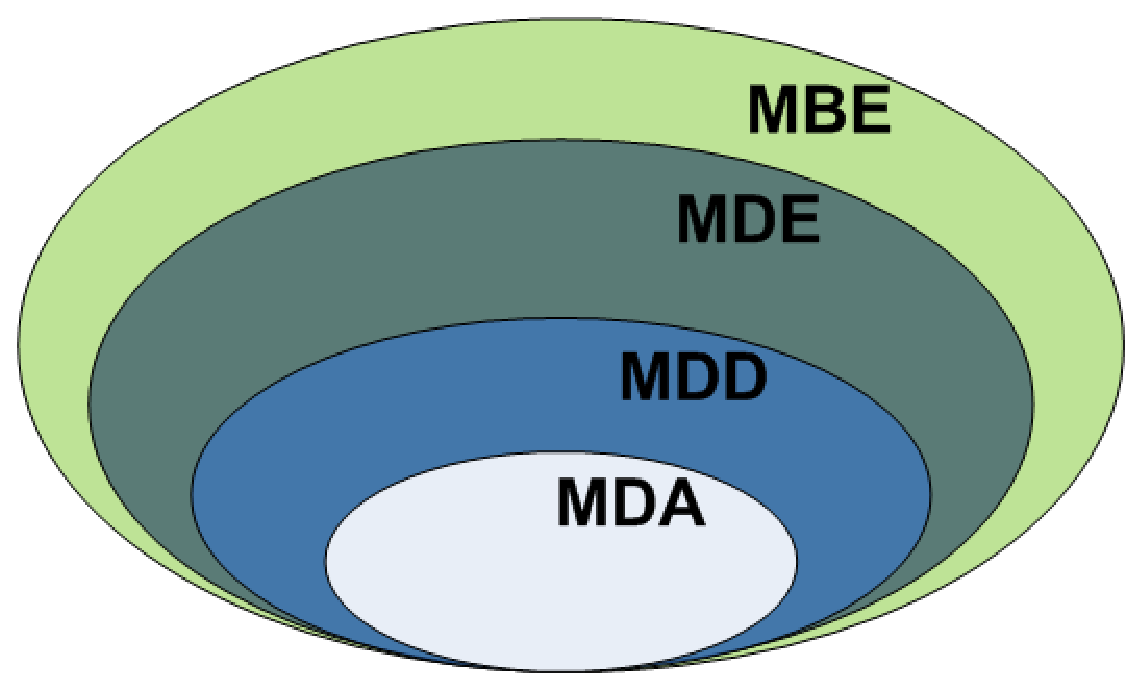
\includegraphics[width=.70\linewidth]{background/images/MDAMDDMDEMBE.eps} \\
  \caption{Capas del modelado de lenguajes}
  \label{back:fig:MDA}
\end{figure}

Tanto MDD como MDE aportan varias ventajas respecto a m�todos de desarrollo tradicionales, podemos encontrar las siguientes ventajas [8], [9]:
\begin{enumerate}
\item Tiempo de desarrollo menor.
\item Reutilizaci�n de componentes en distintos sistemas.
\item Alto nivel de abstracci�n para escribir aplicaciones y artefactos de software a trav�s de la arquitectura de niveles del meta-modelado y las capas de modelado de MDD. Este beneficio favorece dise�ar una aplicaci�n partiendo de lo mas general a lo m�s concreto, es decir, son independientes de la tecnolog�a.
\item Un menor n�mero de l�neas de c�digo escritas, ya que los niveles de abstracci�n que aporta MDD a trav�s de los modelos y meta-modelos dise�ados fomentan el re�so del c�digo y de los modelos.
\item Si se centran los esfuerzos en el generador de c�digo se puede mejorar la calidad del software, adem�s reducimos la cantidad de errores as� como el tiempo dedicado en pruebas e incurrimos en buenas pr�cticas de desarrollo.
\end{enumerate}

Una vez entendidos los conceptos anteriores y los beneficios que nos proporciona este enfoque de desarrollo se presentan los conceptos b�sicos que nos ayudaran a comprender como funciona MDD.

El enfoque MDD parte del meta-modelo [10], un meta-modelo es la representaci�n del lenguaje que se desea implementar en sintaxis abstracta. Un lenguaje de modelado est� formado de sintaxis y sem�ntica. La sintaxis son el conjunto de normas o reglas de escritura del lenguaje. La sem�ntica refleja el significado de la sintaxis.
La definici�n de esta sintaxis abstracta forma parte del primer paso en el proceso de dise�o de un lenguaje, esta sintaxis abstracta especifica la forma del meta-modelo. Clases y relaciones de dominio son los principales elementos que forman parte de un meta-modelo. A su vez los meta-modelos son considerados instancias de estos lenguajes de modelado. Un ejemplo de meta-modelo es la definici�n de UML [11]. En UML por ejemplo elementos como las clases, paquetes o atributos se pueden usar dentro del propio UML.

El siguiente paso consiste en la definici�n de la sintaxis concreta, este paso se basa en la representaci�n de los elementos bien definidos en la sintaxis abstracta, esto es la creaci�n de un modelo. Un modelo es la representaci�n concreta de los elementos descritos en la sintaxis abstracta o meta-modelo. Por lo tanto un modelo siempre posee las propiedades y cumple las restricciones de su meta-modelo. En la figura~\ref{back:fig:ejALL} se pueden observar representaciones de los elementos descritos.

\begin{figure}[!tb]
  \centering
  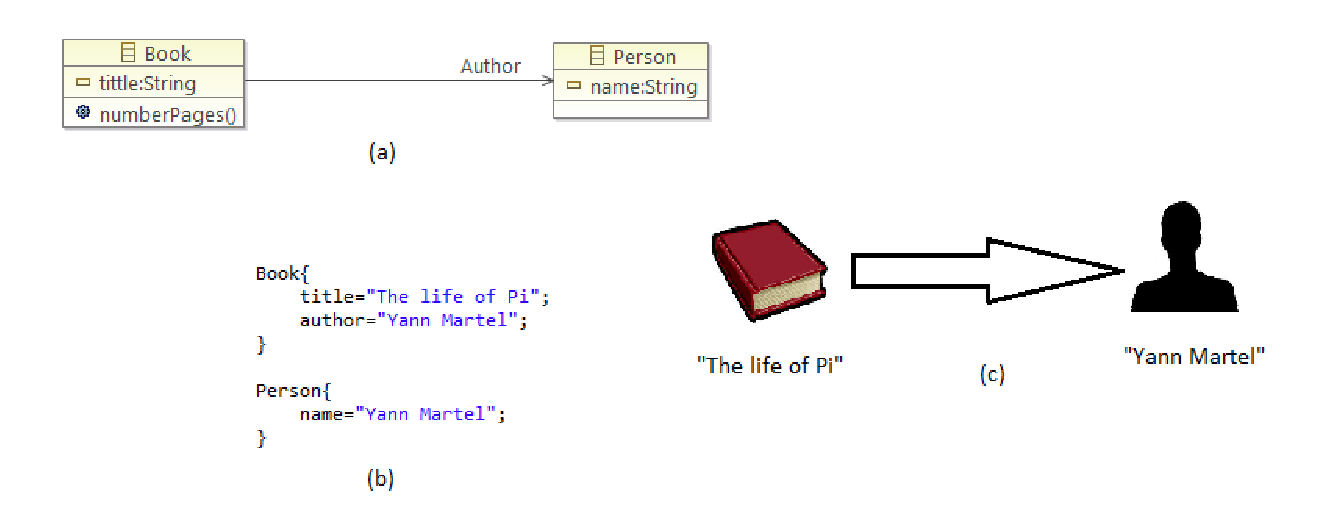
\includegraphics[width=1.1\linewidth]{background/images/ejALL.eps} \\
  \caption{(a) Meta-modelo, (b) Sintaxis concreta, (c) Sintaxis grafica}
  \label{back:fig:ejALL}
\end{figure}

Seg�n [10], formalizando los conceptos anteriores estos son los pasos que hay que realizar para la creaci�n de un nuevo lenguaje de modelado:
\begin{enumerate}
\item En primer lugar hay que establecer cu�l va a ser la sintaxis de nuestro lenguaje de modelado. Para ello hay que crear un meta-modelo el cual como se comentaba anteriormente establece cuales son las reglas que han de seguir los modelos. El meta-modelo ha de ser construido utilizando un lenguaje de meta-modelado, el lenguaje de modelado utilizado en el presente proyecto es ECore [8]. Adem�s de ECore hay otros lenguajes de modelado como puede ser MOF [9].
\item El siguiente paso consiste en la definici�n de la sintaxis concreta de nuestro lenguaje de modelado. La creaci�n de un modelo bien definido a partir del meta-modelo creado en el paso anterior.
\item La definici�n de la sem�ntica del lenguaje de modelado es el �ltimo paso, por ejemplo crear un generador que transforme los elementos del modelo en elementos de un lenguaje distinto bien definido.
\end{enumerate}

La herramienta con la que se va a trabajar para crear el lenguaje de modelado correspondiente a Cassandra es EMF, un plugin de eclipse que nos permite crear y trabajar con lenguajes de modelado.
MDD proporciona las transformaciones de modelos como principal herramienta para trabajar con modelos en el proceso de desarrollo software. Existen dos tipos de transformaciones:
\begin{enumerate}
\item \emph{Model to model (M2M)}. Dado un modelo de entrada esta transformaci�n produce otro modelo como salida. Este tipo de transformaci�n se puede utilizar de varias formas, la primera transformar un modelo d�ndole propiedades que no posee el original. La segunda es la que se utilizara en el presente proyecto, dado un modelo origen definido en UML realizar una transformaci�n a un modelo destino definido en Cassandra (Figura~\ref{back:fig:transformacion}). Esta informaci�n es ampliada en el siguiente cap�tulo.

\item \emph{Model to text (M2T)}. Es la ultima transformaci�n que se realiza en la etapa de desarrollo para la creaci�n del generador de c�digo de la aplicaci�n. Estas transformaciones no generan un modelo de salida sino una representaci�n textual del modelo que se desea transformar. Se puede utilizar para generar por ejemplo una representaci�n del modelo transformado en formato HTML.
\end{enumerate}

\begin{figure}[!tb]
  \centering
  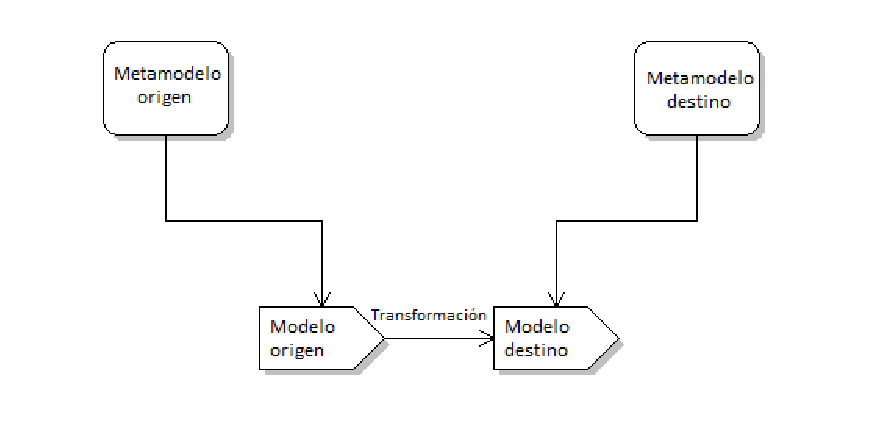
\includegraphics[width=1.05\linewidth]{background/images/transformacion.eps} \\
  \caption{Proceso de transformaci�n de un modelo}
  \label{back:fig:transformacion}
\end{figure}

Para explicar todo este proceso se presenta un sencillo ejemplo donde se explican c�mo se utilizan brevemente las t�cnicas de desarrollo dirigido por modelos, Model to Model (M2M) y Model to Text (M2T). Para aplicar M2M nos har�n falta dos meta-modelos (uno origen y uno destino) y para aplicar M2T se ha dise�ado un sencillo generador de c�digo HTML.

La figura~\ref{back:fig:grafoMetamodelo} muestra la representaci�n de la sintaxis abstracta o meta-modelo del lenguaje. El meta-modelo consiste en un sencillo grafo el cual est� compuesto de un n�mero indefinido de nodos los cuales est�n conectados entre s� mediante aristas. Estos nodos como se ve en la imagen tienen un atributo de tipo "Tcolor" por lo que un Nodo puede ser de color rojo o de color azul. Por lo tanto un modelo bien definido de este meta-modelo ser� un modelo que contenga un grafo con un numero cualquiera de Nodos conectados dos a dos entre s� mediante aristas.

\begin{figure}[!tb]
  \centering
  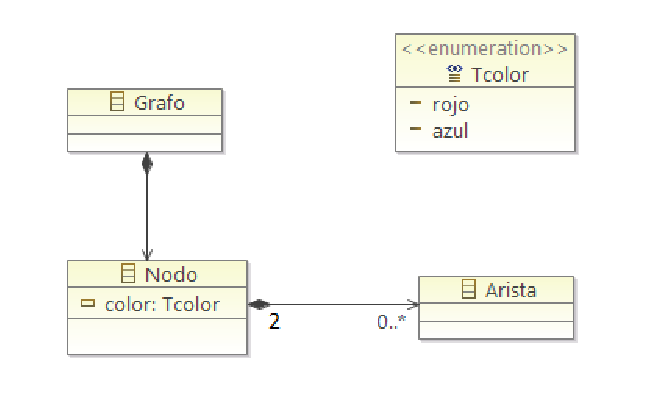
\includegraphics[width=.8\linewidth]{background/images/grafoMetamodelo.eps} \\
  \caption{Meta-modelo de un grafo}
  \label{back:fig:grafoMetamodelo}
\end{figure}

A continuaci�n se presenta otro meta-modelo como se ve en la figura~\ref{back:fig:metamodeloRed}. Este meta-modelo consiste en la representaci�n de una red de computadores que est� compuesta de PC's y Routers estos an�logamente al anterior meta-modelo est�n conectados indistintamente entre s� mediante cables. Tanto los nodos como los cables tiene un atributo de tipo "String" para definir el nombre.

\begin{figure}[!tb]
  \centering
  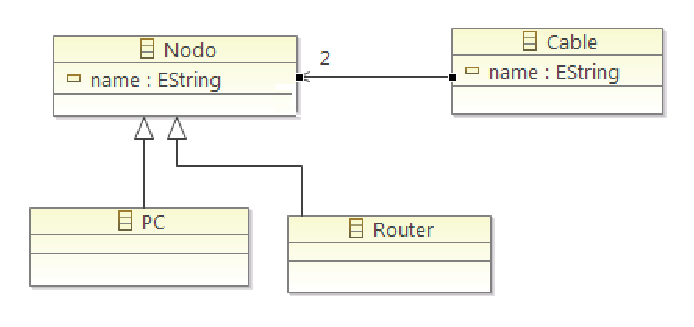
\includegraphics[width=.8\linewidth]{background/images/metamodeloRed.eps} \\
  \caption{Meta-modelo de una red}
  \label{back:fig:metamodeloRed}
\end{figure}

Nuestro objetivo es la transformaci�n de un modelo de tipo Grafo a un modelo de tipo Red, dependiendo del color del Nodo, el Nodo ser� transformado en un PC o en un Router (Rojo-PC, Azul-Router) para realizar esta transformaci�n se utilizan t�cnicas M2M.

Una vez obtenido el modelo de tipo Red deseamos representar textualmente el modelo generado para ello utilizamos t�cnicas M2T. En este caso la representaci�n del modelo es realizada en formato HTML. La representaci�n del c�digo generado utilizando un modelo de tipo grafo y aplicando la transformaci�n entre modelos es el que se puede observar en la figura~\ref{back:fig:ejGeneradorHTML}.

\begin{figure}[!tb]
  \centering
  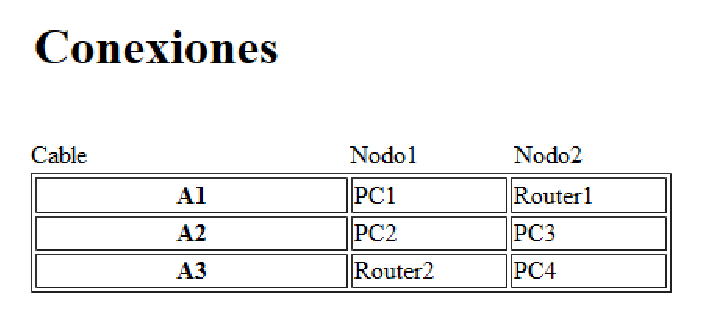
\includegraphics[width=.8\linewidth]{background/images/ejGeneradorHTML.eps} \\
  \caption{Resultado transformaci�n HTML}
  \label{back:fig:ejGeneradorHTML}
\end{figure}

El proceso que se ha seguido es explicado m�s detalladamente en cap�tulos posteriores con un caso de estudio analizado, tanto las t�cnicas de transformaci�n de modelos como la realizaci�n del generador de c�digo as� como la creaci�n de los modelos.





\section{Motivaci�n y Objetivos}
\label{sec:intr:objetivos}

%%==================================================================%%
%% Author : Sa�udo Olmedo, Ignacio                                  %%
%%          S�nchez Barreiro, Pablo                                 %%
%% Version: 1.4, 18/06/2013                                         %%                                                                                    %%                                                                  %%
%% Memoria del Proyecto Fin de Carrera                              %%
%% Introduccion/Motivaci�n y objetivos                              %%
%%==================================================================%%



Como hemos visto a lo largo de la introducci�n el enfoque que proporciona el Desarrollo Dirigido por Modelos as� como la Ingenier�a Dirigida por Modelos nos proporciona m�ltiples ventajas respecto al desarrollo tradicional por lo que la utilizaci�n de este enfoque es apropiada para la realizaci�n del generador de c�digo as� como para las transformaciones entre modelos.

La utilizaci�n de modelos UML respecto a modelos escritos en Cassandra a la hora de especificar una base de datos no relacional proporciona una abstracci�n para aquellos usuarios que no est�n muy familiarizados con el modelado de bases de datos no relacionales. Por lo que la utilizaci�n de modelos escritos en UML es ventajosa ya que UML es un lenguaje de modelado bien conocido por toda la comunidad de dise�adores.

Como se comenta al inicio del documento, el objetivo de este proyecto de fin de carrera es la implementaci�n de un generador de c�digo que transforme un modelo UML en su correspondiente c�digo ejecutable en Cassandra. Previa implementaci�n del generador de c�digo habr� que transformar el modelo UML a un modelo escrito en Cassandra. Para ello necesitaremos contar con el metamodelo de Cassandra-CQL y el metamodelo de UML. Dicho generador y dicha transformaci�n se desarrollaran utilizando el enfoque y las t�cnicas que proporcionan el Desarrollo Dirigido por Modelos. Esta implementaci�n ser� realizada con el framework que proporciona eclipse de modelado llamado EMF.

Como resultado del proyecto se genera un c�digo escrito en el lenguaje de Cassandra (CQL-Cassandra Query Language) que puede ser ejecutado en cualquier herramienta que soporte dicho lenguaje.




\section{Estructura del Documento}
\label{sec:intr:estructura}

%%==================================================================%%
%% Author : Sa�udo Olmedo, Ignacio                                  %%
%%          S�nchez Barreiro, Pablo                                 %%
%% Version: 1.3, 18/06/2014                                         %%                                                                                    %%                                                                  %%
%% Memoria del Proyecto Fin de Carrera                              %%
%% Introducci�n/Roadmap                                             %%
%%==================================================================%%


Tras este cap�tulo de introducci�n, la presente memoria del Proyecto Fin de Carrera se estructura tal y como se describe a continuaci�n: El Capitulo 2 describe en t�rminos generales todos los conceptos y tecnolog�as que son necesarios para comprender el contenido de esta memoria conceptos tales como Cassandra o EMF por ejemplo. El Capitulo 3 describe como se ha realizado la transformaci�n de modelos as� como la metodolog�a de transformaci�n de modelos (M2M). El Cap�tulo 4 describe como se ha realizado el generador de c�digo as� como las t�cnicas y tecnolog�as utilizadas. Finalmente el Cap�tulo 5 presenta mis conclusiones tras la realizaci�n del proyecto as� como posibles mejores de la herramienta. (Puede cambiar). 


